
\documentclass[11pt,fleqn]{article}
\usepackage[margin=1in,top=1in,bottom=1in]{geometry}
\usepackage{mathtools}
\usepackage{longtable}
\usepackage{enumitem}
\usepackage{hyperref}
\usepackage[dvips]{graphics}
\usepackage[table]{xcolor}
\usepackage{amssymb}
\usepackage{subfig}
\usepackage{booktabs}
\usepackage{tikz}

\usepackage[normalem]{ulem}

\usepackage{multicol}
\usepackage{txfonts}
%\usepackage{amsfonts}
\usepackage{natbib}

\usepackage{gb4e}
%\usepackage{/Users/judith/Library/Latex/drs}
%\usepackage{/Users/judith/Library/Latex/avm}
\usepackage[all]{xy}
\usepackage{rotating}
\usepackage{tipa}
\usepackage{multirow}
\usepackage{authblk}
\usepackage{adjustbox}
\usepackage{array}


\newcolumntype{R}[2]{%
    >{\adjustbox{angle=#1,lap=\width-(#2)}\bgroup}%
    l%
    <{\egroup}%
}
\newcommand*\rot{\multicolumn{1}{R{60}{1em}}}% no optional argument here, please!

\newcommand{\foc}{$_{\mbox{\small F}}$}
\newcommand{\lp}{<_{\hspace*{-.1cm}p}}
\newcommand{\lnai}{<_{\hspace*{-.1cm}nai}}

\setlength{\parindent}{.8cm}
\setlength{\parskip}{0ex}
\setlength{\headsep}{0in}

\setlength{\bibsep}{0mm}
\bibpunct[:]{(}{)}{;}{a}{,}{,}

\newcommand{\yi}{\'{\symbol{16}}}
\newcommand{\nasi}{\~{\symbol{16}}}
\newcommand{\hina}{h\nasi na}
\newcommand{\ina}{\nasi na}
%\renewcommand{\abut}{$\supset$\hspace*{-0.07cm}$\subset$}
\newcommand{\tto}{t$_{top}$}
\newcommand{\wtop}{w$_{top}$}
\newcommand{\tc}{t$_c$}
\newcommand{\schwa}{\begin{sideways}e\end{sideways}}

% Semantic brackets
%\newcommand{\iss}[1]{\mbox{\protect\tiny \mbox{#1}}}
%\newcommand{\sem}[2]{\6#1\9$_\iss{#2}$} David's original
\newcommand{\6}{\mbox{$[\hspace*{-.6mm}[$}} 
\newcommand{\9}{\mbox{$]\hspace*{-.6mm}]$}}
\newcommand{\sem}[2]{\6#1\9$^{#2}$}

\newcommand{\semt}[2]{$\left[\hspace*{-.6mm}\left[\begin{tabular}[c]{@{}l@{}}#1\vspace*{-.5em}\end{tabular}\right]\hspace*{-.6mm}\right]\hspace*{-.6mm}^{#2}$}

\renewcommand{\baselinestretch}{1}

\def\bad{{\leavevmode\llap{*}}}
\def\marginal{{\leavevmode\llap{?}}}
\def\verymarginal{{\leavevmode\llap{??}}}
\def\infelic{{\leavevmode\llap{\#}}}

\definecolor{Lighter}{gray}{.92}
\definecolor{Blue}{RGB}{0,0,255}
\definecolor{Green}{RGB}{10,200,100}
\definecolor{Red}{RGB}{255,0,0}


\newcommand{\citepos}[1]{\citeauthor{#1}'s \citeyear{#1}}
\newcommand{\citeposs}[1]{\citeauthor{#1}'s}
\newcommand{\citetpos}[1]{\citeauthor{#1}'s (\citeyear{#1})}

\newcommand{\eref}[1]{(\ref{#1})}
\newcommand{\tableref}[1]{Table \ref{#1}}
\newcommand{\figref}[1]{Fig.~\ref{#1}}
\newcommand{\appref}[1]{Appendix \ref{#1}}
\newcommand{\sectionref}[1]{section \ref{#1}}


\title{Prior, probability, projectivity\thanks{This work was partially supported by NSF grant BCS-1452674 (JT).}}

%\author[$\bullet$]{Judith Tonhauser}
%\author[$\triangleright$]{Judith Degen}
%
%\affil[$\bullet$]{The Ohio State University}
%\affil[$\triangleright$]{Stanford University}

%\renewcommand\Authands{ and }
%
%\newcommand{\jt}[1]{\textbf{\color{blue}JT: #1}}
%\newcommand{\jd}[1]{\textbf{\color{Green}[jd: #1]}}  

\begin{document}

\maketitle

\begin{abstract}
abstract
\end{abstract}

%\tableofcontents

%\newpage
			
\section{Introduction}\label{s1}

\citealt*{tbd-variability}

\section{Pre-tests}\label{s-pretests}

\footnote{\label{f-github}The
data and R code for generating the figures and analyses
of the experiments reported on in this paper are available at \url{https://github.com/judith-tonhauser/projective-probability}.}

\subsection{Event probability pretest}\label{s-pretest1}

\subsubsection{Methods}\label{s-methods-1}

\paragraph{Participants.} 95 participants with U.S.\ IP addresses and at least 99\% of previous HITs approved were recruited on Amazon's Mechanical Turk platform (ages: 21-75; median: 33; 45 female, 50 male). They were paid 55 cents for participating in the experiment. 

\paragraph{Materials.} The prior probability of 20 events described by English sentences were explored in this experiment. Each of the 20 event descriptions was paired with two facts about the world, described by English sentences and labeled `Fact:', for a total of 40 fact/event pairs. Each event was hypothesized to be relatively more likely given one of the two facts than given the other fact that the event was paired with. Two fact/event pairs are given in (\ref{event}) for the event described by the English sentence {\em Mary is pregnant}: this event was hypothesized to be more likely given the fact described in (\ref{event1}i) than given the fact described in (\ref{event2}i). See Appendix \ref{a-exp1} for the other 19 event descriptions and the fact descriptions that the event descriptions were paired with.\footnote{Need to say that we use `event' for events and states, rather than `eventuality'.}

\begin{exe}
\ex\label{event}
\begin{xlist}
\ex\label{event1}
\begin{xlist}
\ex Fact: Mary is taking a prenatal yoga class
\ex Mary is pregnant
\end{xlist}
\ex\label{event2}
\begin{xlist}
\ex Fact: Mary is a middle school student
\ex Mary is pregnant
\end{xlist}
\end{xlist}
\end{exe}

{\bf fact/event pairs were chosen so that neither at ceiling nor at floor. We need to avoid eventualities being too likely or too unlikely, given their two facts, because a) if they are too likely, then people might argue that the facts of the world entail the content of the clause describing the eventuality, and b) if they are too unlikely, then participants might give wonky projectivity ratings.}

The experiment also included two control stimuli, which were used to assess whether participants were attending to the task. Like the target stimuli, both control stimuli consisted of a sentence describing a fact about the world and a sentence describing an event, as shown in (\ref{control1}) and (\ref{control2}). The two control stimuli differ in the probability of the event given the fact about the world: whereas the event of Barry living in Europe has a probability of 1, given the fact that Barry lives in Germany, the event of Tammy speaking Italian and Greek has a probability of 0, given that Tammy is a rabbit. 

\begin{exe}
\ex\label{control1}
\begin{xlist}
\exi{i.} Fact: Barry lives in Germany 
\exi{ii.} Barry lives in Europe 
\end{xlist}
\ex\label{control2}
\begin{xlist}
\exi{i.} Fact: Tammy is a rabbit 
\exi{ii.} Tammy speaks Italian and Greek 
\end{xlist}
\end{exe}

The 40 target stimuli were distributed across two lists of 20 target stimuli each so that each list contained 20 unique event descriptions and each list included 10 fact/event pairs for which the event was hypothesized to be likely and 10 fact/event pairs for which the event was hypothesized to be less likely. The two control stimuli were added to each list, for a total of 22 stimuli per list. 

\paragraph{Procedure.} Participants were randomly assigned to a list. They were told that they would read a fact about the world and were asked to assess how likely a particular event was, given the fact. The 22 stimuli were presented in random order to each participant. On each trial, participants read the fact and the corresponding response question, which was formed from {\em How likely is it that\ldots ?} with the sentence describing the event realizing the embedded clause of the question. Participants gave their response on a slider marked `impossible' at one end (coded as 0) and `definitely' at the other (coded as 1), as shown in \figref{f-trial-exp1}. 

\begin{figure}[h!]
\begin{center}
\fbox{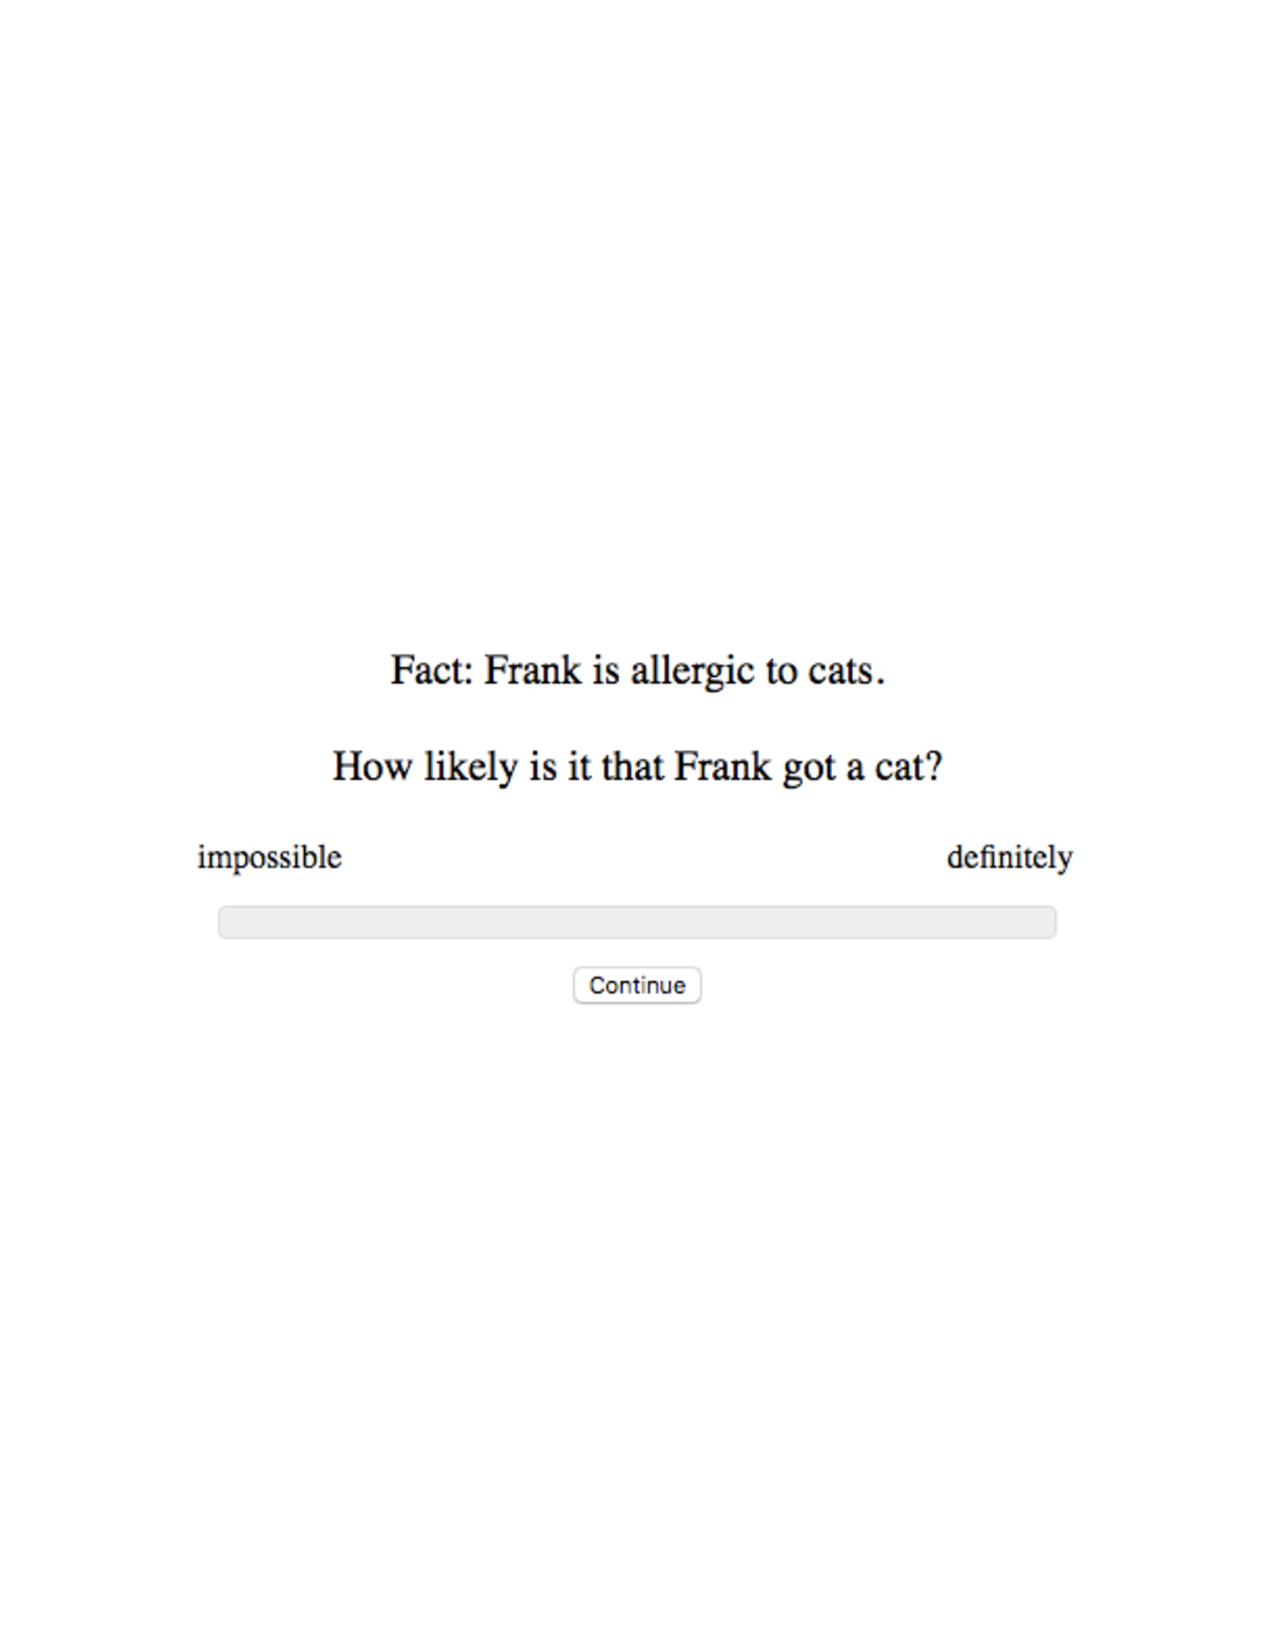
\includegraphics[width=8cm]{figures/exp1a-trial}}
\end{center}
\caption{A sample trial in Exp.~1}\label{f-trial-exp1}
\end{figure}

After completing the experiment, participants filled out a short optional survey about their age, their gender, their native language(s) and, if English is their native language, whether they are a speaker of American English (as opposed to, e.g., Australian or Indian English). To encourage them to respond truthfully, participants were told that they would be paid no matter what answers they gave in the survey. 

\paragraph{Data exclusion.}
Prior to analysis, the data from 8 participants who did not self-identify as native speakers of American English were excluded. For the remaining 87 participants, we inspected their responses to the two control stimuli (the group means were .86 for (\ref{control1}) and .03 for (\ref{control2})). 19 participants gave responses lower than .8 to (\ref{control1}) or responses higher than .2 to (\ref{control2}), suggesting that these participants did not attend to the task or interpreted the task differently. The data from these 19 participants were also excluded, leaving data from 68 participants (ages 21-75; median: 36; 31 female, 37 male).  

\subsubsection{Results and discussion}

As expected, likeliness ratings of events were influenced by facts about the world: overall, the mean likeliness rating for events presented with facts that make the event more likely was .7 (sd = .21) and the mean likeliness rating for events presented with facts that make the event less likely was .16 (sd = .17). Figure \ref{f-priors} shows the likeliness rating for the 20 events given facts that make the events more likely (brown dots) and facts that make the events less likely (blue dots). Mean likeliness ratings for each of the 40 fact/event pairs are shown as black dots. Error bars indicate 95\% confidence intervals.

\begin{figure}[h!]
\centering

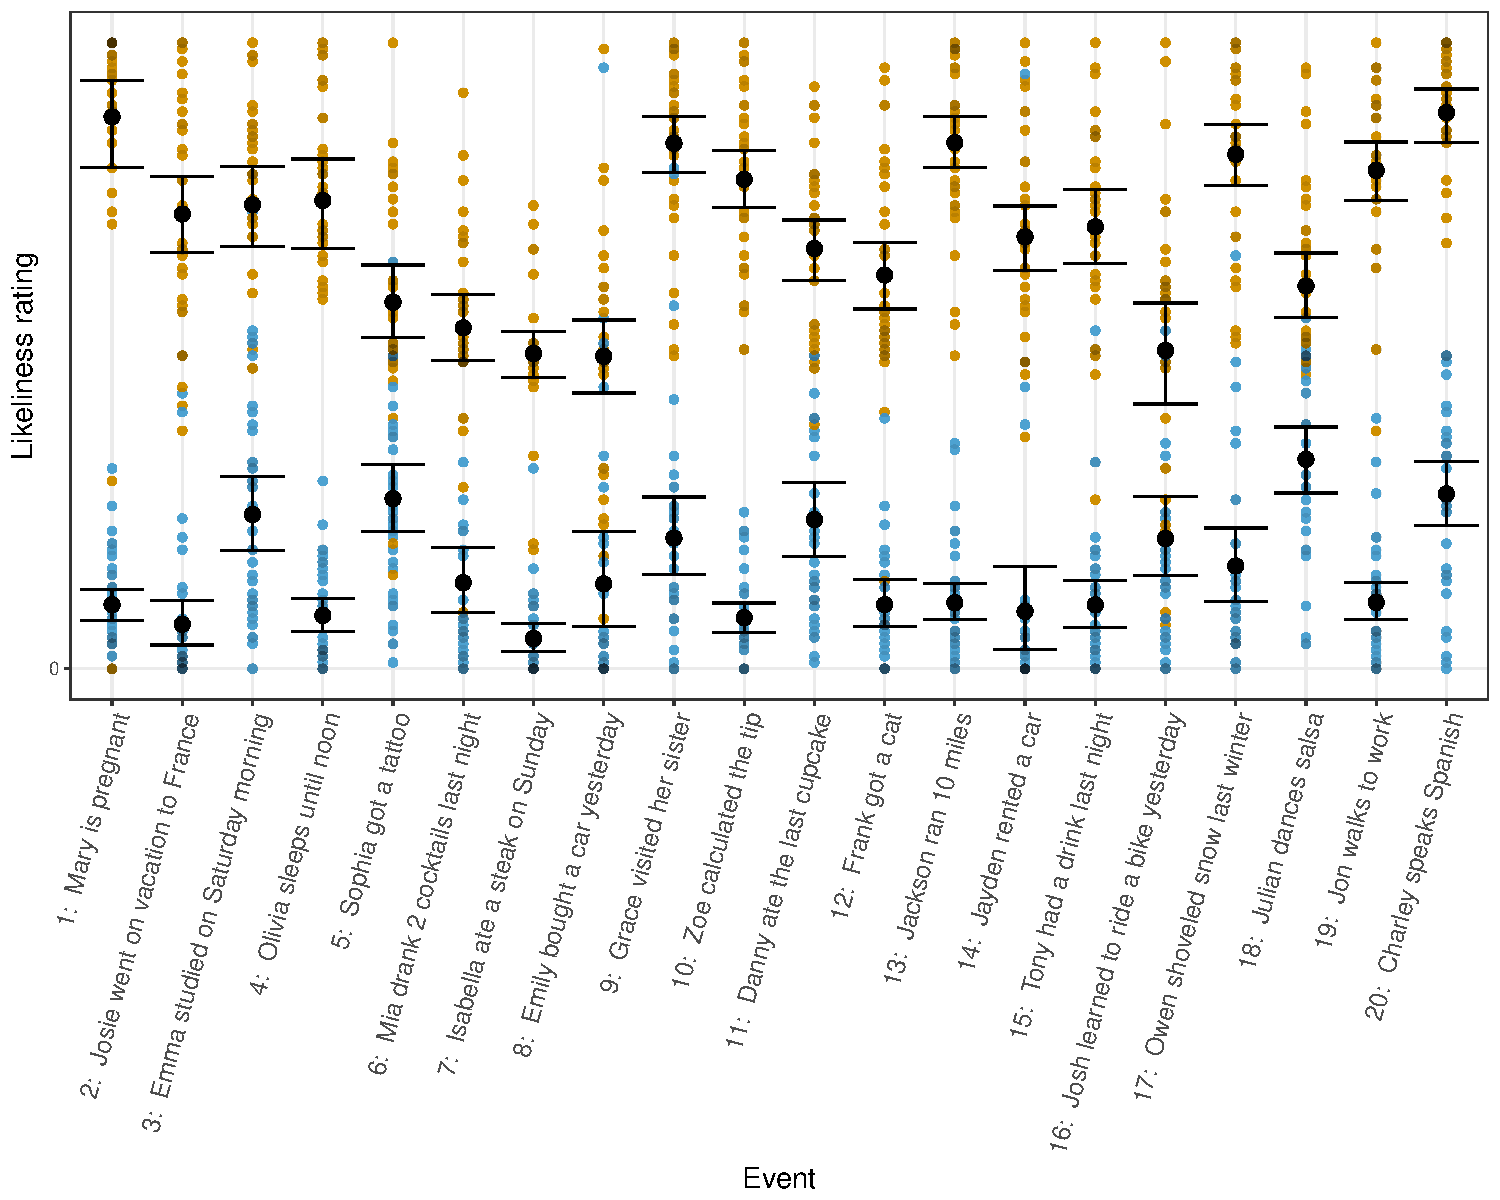
\includegraphics[width=.8\paperwidth]{../results/1-prior/graphs/target-ratings}

\caption{Likeliness ratings for 20 events given facts about the world that make the events more likely (brown dots) and facts about the world that make the events less likely (blue dots); darker dots indicate overlapping ratings. Mean likeliness ratings for the 40 fact/event pairs are given by black dots. Error bars indicate 95\% confidence intervals.}\label{f-priors}
\end{figure}

For each event, the likeliness of the event is higher given the fact that makes the event more likely than given the fact that makes the event less likely. At the same time, the likeliness of none of the events given a particular fact is at ceiling or at floor. We have thus succeeded in identifying suitable fact/fact/event triples for our study of how projectivity is influenced by event probability.

\subsection{Entailment pretest}\label{s-pretest2}

\subsubsection{Methods}\label{s-methods-2}

\paragraph{Participants.} XX participants with U.S.\ IP addresses and at least 99\% of previous HITs approved were recruited on Amazon's Mechanical Turk platform (ages: XX-XX; median: XX). They were paid XX cents for participating in the experiment. 

\paragraph{Materials.} 

\paragraph{Procedure.} Participants were told that they would read a fact about the world and were asked to assess how likely a particular event was, given the fact. On each trial participants read the fact and the corresponding response question, and then gave their response on a slider marked `impossible' at one end and `definitely' at the other, as shown in \figref{f-trial-exp1}.  

\begin{figure}[h!]
\begin{center}
\fbox{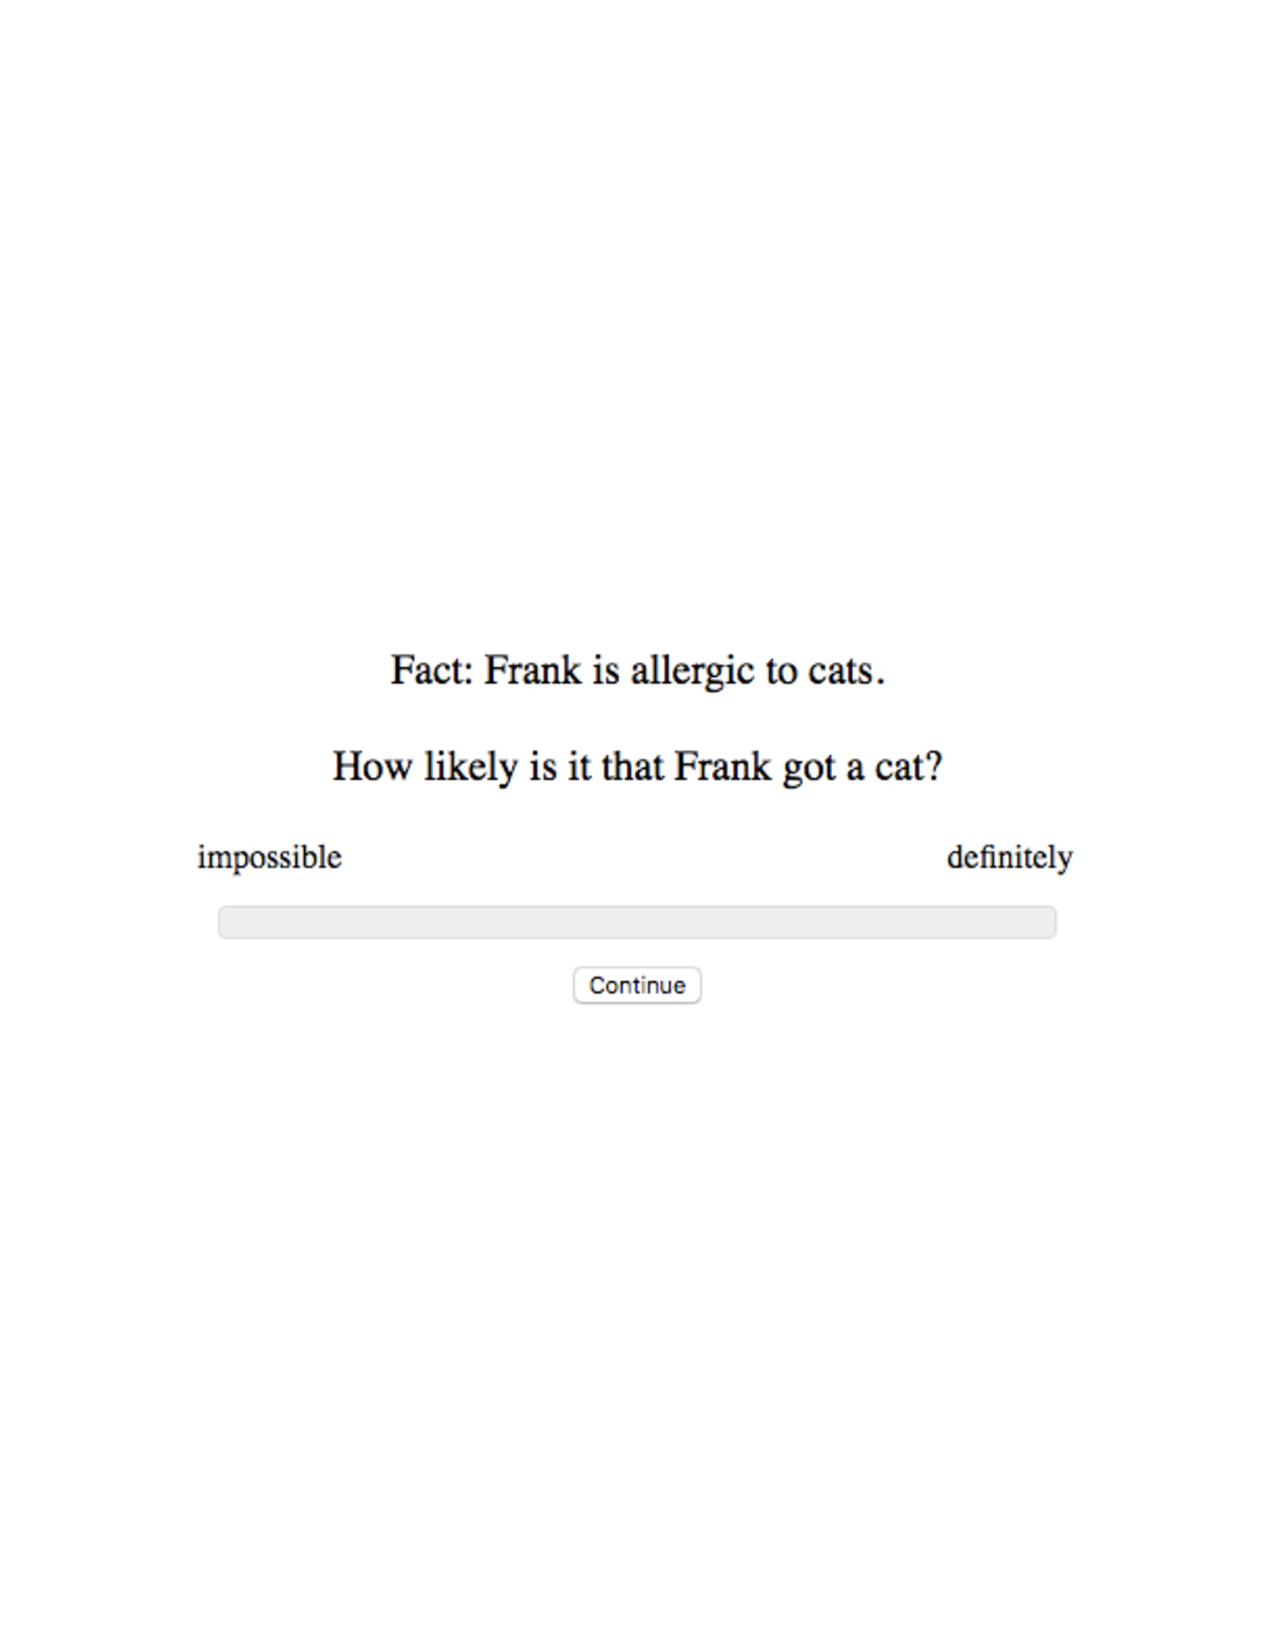
\includegraphics[width=8cm]{figures/exp1a-trial}}
\end{center}
\caption{A sample trial in Exp.~2}\label{f-trial-exp1}
\end{figure}

After completing the experiment, participants filled out a short optional survey about their age, their gender, their native language(s) and, if English is their native language, whether they are a speaker of American English (as opposed to, e.g., Australian or Indian English). To encourage them to respond truthfully, participants were told that they would be paid no matter what answers they gave in the survey.

\paragraph{Data exclusion.}
Prior to analysis, the data from XX participants who did not self-identify as native speakers of American English were excluded. For the remaining XX participants, we inspected their responses to the two control stimuli. XX participants...., suggesting that these participants did not attend to the task or interpreted the task differently. The data from these XX participants were also excluded, leaving data from XX participants (ages XX-XX; median: XX).  

\subsubsection{Results and discussion}

\begin{figure}[h!]
\centering

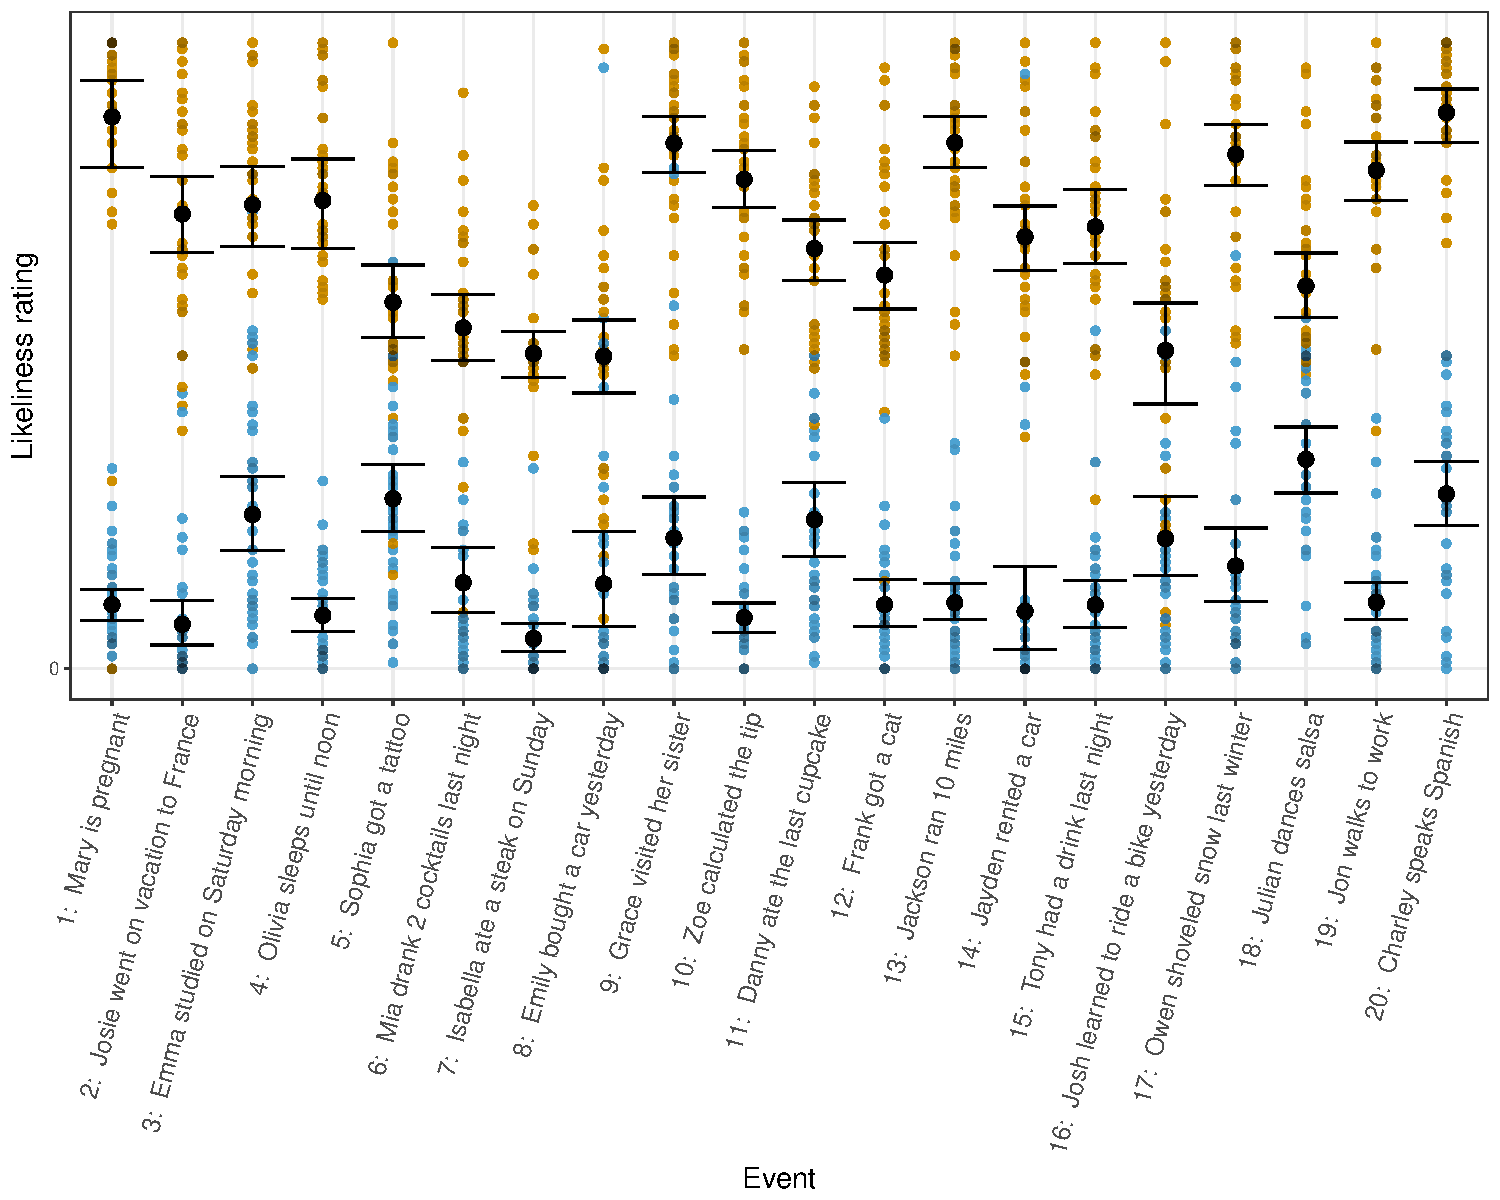
\includegraphics[width=.8\paperwidth]{../results/1-prior/graphs/target-ratings}

\caption{Entailment}\label{f-priors}
\end{figure}

\subsection{Interim summary}

\section{Projection experiment}

\section{Conclusions}\label{s6}


\appendix

\setcounter{table}{0}
\renewcommand{\thetable}{A\arabic{table}}

\setcounter{figure}{0}
\renewcommand{\thefigure}{A\arabic{figure}}

\section{Materials used in Exp 1}\label{a-exp1}

The 20 event descriptions used in the event probability pretest; facts about the world that make the event more (H) or less likely (L) are given in parentheses. 

\begin{enumerate}[leftmargin=3ex,itemsep=-2pt]
\item Mary is pregnant (Mary is a middle school student / Mary is taking a prenatal yoga class)
\item Josie went on vacation to France (Josie doesn't have a passport / Josie loves France)
\item Emma studied on Saturday morning (Emma is in first grade / Emma is in law school)
\item Olivia sleeps until noon (Olivia has two small children / Olivia works the third shift)
\item Sophia got a tattoo (Sophia is a high end fashion model / Sophia is a hipster)
\item Mia drank 2 cocktails last night (Mia is a nun / Mia is a college student)
\item Isabella ate a steak on Sunday (Isabella is a vegetarian / Isabella is from Argentina)
\item  Emily bought a car yesterday (Emily never has any money / Emily has been saving for a year)
\item  Grace visited her sister (Grace hates her sister / Grace loves her sister)
\item Zoe calculated the tip (Zoe is 5 years old / Zoe is a math major)
\item  Danny ate the last cupcake (Danny is a diabetic / Danny loves cake)
\item  Frank got a cat (Frank is allergic to cats / Frank has always wanted a pet)
\item  Jackson ran 10 miles (Jackson is obese / Jackson is training for a marathon)
\item  Jayden rented a car (Jayden doesn't have a driver's license / Jayden's car is in the shop)
\item  Tony had a drink last night (Tony has been sober for 20 years / Tony really likes to party with his friends)
\item  Josh learned to ride a bike yesterday (Josh is a 75-year old man / Josh is a 5-year old boy)
\item  Owen shoveled snow last winter (Owen lives in New Orleans / Owen lives in Chicago)
\item  Julian dances salsa (Julian is German / Julian is Cuban)
\item  Jon walks to work (Jon lives 10 miles away from work / Jon lives 2 blocks away from work)
\item  Charley speaks Spanish (Charley lives in Korea / Charley lives in Mexico)
\end{enumerate}

\clearpage

\section{Materials used in Exp 2}\label{a-exp2}

\section{Materials used in Exp 3}\label{a-exp3}

\bibliographystyle{cslipubs-natbib}
\bibliography{bibliography}


\end{document}
